\documentclass[11pt]{article}

\usepackage[T1]{fontenc}
\usepackage{lmodern}
\usepackage{amsmath,amssymb,amsthm,mathtools}
\usepackage{microtype}
\usepackage[margin=1in]{geometry}
\usepackage{booktabs}
\usepackage{array}
\usepackage{longtable}
\usepackage{enumitem}
\usepackage{xcolor}
\usepackage{listings}
\usepackage{graphicx}
\usepackage{caption}
\usepackage{hyperref}
\usepackage{cleveref}
\usepackage{url}

\hypersetup{
  colorlinks=true,
  linkcolor=blue!45!black,
  urlcolor=blue!45!black,
  citecolor=blue!45!black,
  pdftitle={Contender 20: Second-Order Diagonal Hyperreflection in BusyLean},
  pdfauthor={BusyLean research package}
}

\definecolor{codebg}{RGB}{248,248,248}
\definecolor{codeframe}{RGB}{205,205,205}
\definecolor{commentgray}{RGB}{90,90,90}

\lstdefinelanguage{lean}{
  keywords={abbrev,def,theorem,inductive,structure,where,match,with,fun,let,in,
    namespace,end,open,import,by,have,show,exact,intro,apply,constructor,change},
  sensitive=true,
  morecomment=[l]{--},
  morecomment=[s]{/-}{-/},
  morestring=[b]",
}
\lstset{
  language=lean,
  basicstyle=\ttfamily\footnotesize,
  keywordstyle=\bfseries\color{blue!45!black},
  commentstyle=\itshape\color{commentgray},
  stringstyle=\color{green!35!black},
  columns=fullflexible,
  keepspaces=true,
  breaklines=true,
  breakatwhitespace=false,
  showstringspaces=false,
  frame=single,
  framerule=0.35pt,
  rulecolor=\color{codeframe},
  backgroundcolor=\color{codebg},
  xleftmargin=0.8em,
  xrightmargin=0.8em,
  aboveskip=0.7em,
  belowskip=0.7em,
  literate={→}{{$\to$}}1 {←}{{$\leftarrow$}}1 {∀}{{$\forall$}}1
    {≤}{{$\le$}}1 {<}{{$<$}}1 {∧}{{$\wedge$}}1 {⟨}{{$\langle$}}1
    {⟩}{{$\rangle$}}1 {₀}{{$_0$}}1 {₁}{{$_1$}}1 {₂}{{$_2$}}1
}

\newtheorem{theorem}{Theorem}[section]
\newtheorem{lemma}[theorem]{Lemma}
\newtheorem{proposition}[theorem]{Proposition}
\newtheorem{corollary}[theorem]{Corollary}
\theoremstyle{definition}
\newtheorem{definition}[theorem]{Definition}
\newtheorem{construction}[theorem]{Construction}
\theoremstyle{remark}
\newtheorem{remark}[theorem]{Remark}
\newtheorem{warning}[theorem]{Warning}

\newcommand{\N}{\mathbb{N}}
\newcommand{\lean}[1]{\nolinkurl{#1}}
\newcommand{\leancode}[1]{\texttt{\detokenize{#1}}}
\newcommand{\Fam}{\mathsf{Family}}
\newcommand{\Tr}{\mathsf{Transformer}}
\newcommand{\TL}{\mathsf{TransformerLift}}
\newcommand{\HL}{\mathsf{HyperLift}}
\newcommand{\Prog}{\mathsf{Progressive}}
\newcommand{\Good}{\mathsf{GoodLift}}
\newcommand{\Fnineteen}{F_{19}}
\newcommand{\Ftwenty}{F_{20}}

\title{\textbf{Contender 20: Second-Order Diagonal Hyperreflection in BusyLean}\\[0.4em]
  \large A constructive type-level jump beyond the large-Veblen contender}
\author{Research proposal for the BusyLean project}
\date{13 October 2026}

\begin{document}
\maketitle

\begin{abstract}
BusyLean is a Lean~4 version of the ``name the biggest number'' contest: every
entry is a closed computable natural number and every victory claim is a formal
strict inequality. At the audited baseline, Contender~19 combines a
large-Veblen-length ladder of strongly normalizing object languages with a
natural-rank hierarchy of \emph{transformer lifts}. This article proposes
Contender~20, whose main novelty is not a longer ordinal notation and not one
more numerical iteration, but a jump in the \emph{type of the amplifier}.

We introduce a \emph{hyperlift}, an endomorphism of transformer lifts. We define
countable splicing of lifts, W-tree traversal by an arbitrary hyperlift, an
autonomous second-order lift, and a diagonal hierarchy of hyperlifts. The
proofs isolate a reusable invariant: a good lift both preserves progressive
transformers and strictly exceeds its input transformer. The second-order
hierarchy preserves good lifts and strictly exceeds its base lift, without any
monotonicity assumption on oracle reflection.

At each input $n$, the new function first embeds a complete first-order
hyperreflection layer of rank $\operatorname{family}_{19}(n)+1$ and then applies
a second-order diagonal hierarchy of the same rank. The formal comparison is
factored through the explicit chain
\[
  \operatorname{family}_{19}(n)
  < \operatorname{firstOrder}_{20}(n)
  < F_{20}(n).
\]
Consequently the proposed closed number
\[
  \operatorname{contender}_{20}=F_{20}(F_{20}(42))
\]
strictly exceeds Contender~19. All new definitions are structural and
computable. The package includes Lean source, comparison theorems, a repository
patch, a smoke test, a static constructivity audit, and this compiled article.
The LaTeX and static audits were executed; a Lean~4.34.0 kernel build remains a
required pre-merge step because that toolchain was unavailable in the package
generation environment.
\end{abstract}

\tableofcontents

%======================================================================
\section{Problem, baseline, and result}

\subsection{The contest rule}

The governing principle is stronger than merely writing an expression that is
obviously enormous. A valid contender must satisfy three requirements.

\begin{enumerate}[leftmargin=*]
\item It is a closed Lean term of type \lean{Nat}.
\item It is computable in principle: no appeal to a Busy Beaver, an unbounded
  search whose termination is postulated, or classical choice.
\item Its superiority over the incumbent is certified by a theorem accepted by
  Lean's kernel.
\end{enumerate}

The values in question must never be evaluated. Their magnitude is established
extensionally, through generic strict-growth lemmas whose proof terms are small.
That distinction---huge definitions but small comparison proofs---is central to
BusyLean's engineering.

\subsection{Audited repository state}

This package was designed against the BusyLean \lean{main} tree at commit
\begin{center}
\small\lean{64d31a0cf6f1aa4477a088be5554957de6e87a61}.
\end{center}
The repository pins Lean \lean{v4.34.0}. Its README names Contender~19 as the
current entry. In condensed form, the incumbent is

\begin{lstlisting}
def family18 (n : Nat) : Nat := F18 (F18 n)
def F19 (n : Nat) : Nat :=
  diagonalLift (schedule19 n) (family18 n + 1)
    lTransformer (fun _ => family18) n n
def contender_19 : Nat := F19 (F19 42)
\end{lstlisting}

The object-language component, \lean{lTransformer}, reflects programs in a
ladder whose atoms are Sch\"utte-style large-Veblen terms. The amplifier
component, \lean{diagonalLift}, is a hierarchy of endomorphisms of transformers.
The repository proves

\begin{lstlisting}
theorem contender_18_lt_contender_19 :
  contender_18 < contender_19
\end{lstlisting}

and, more strongly, pointwise domination of the entire predecessor family.

\subsection{Proposed result}

The proposal adds one new amplification level:

\begin{center}
\begin{tabular}{>{\raggedright\arraybackslash}p{0.24\linewidth}
                >{\raggedright\arraybackslash}p{0.31\linewidth}
                >{\raggedright\arraybackslash}p{0.35\linewidth}}
\toprule
Level & Carrier & Intended action\\
\midrule
0 & oracle families & supply numerical data to reflected programs\\
1 & transformers & map oracle families to stronger families\\
2 & transformer lifts & map transformers to stronger transformers\\
3 & hyperlifts & map whole transformer-lift hierarchies to stronger ones\\
\bottomrule
\end{tabular}
\end{center}

Contender~19 reaches Level~2. Contender~20 diagonalizes at Level~3. Its key
formal statements are

\begin{lstlisting}
theorem family19_lt_firstOrder20 (n : Nat) :
  family19 n < firstOrder20 n

theorem firstOrder20_lt_F20 (n : Nat) :
  firstOrder20 n < F20 n

theorem contender_19_lt_contender_20 :
  contender_19 < contender_20
\end{lstlisting}

The intermediate \lean{firstOrder20} is deliberate. It makes the structural
margin visible inside the formal proof: before the second-order hierarchy does
anything, the construction has already performed a complete first-order
\lean{diagonalLift} using a predecessor-sized schedule and rank.

%======================================================================
\section{Why a type-level jump is the right next move}

Several simpler definitions would win the literal comparison but would not be
serious successors.

\subsection{Trivial and near-trivial victories}

The definitions
\[
  \operatorname{contender}_{19}+1,
  \qquad
  F_{19}(F_{19}(F_{19}(42))),
  \qquad
  \text{or}\qquad
  F_{19}^{k}(42)
\]
for some fixed $k$ are computable and easy to compare. They add no new
mathematical mechanism. BusyLean's accepted sequence has consistently sought a
new language, a new reflection principle, a longer well-founded universe
ladder, or a new operator-level closure. Merely inserting another numeral or
another fixed composition would be contrary to that trajectory.

\subsection{A longer ordinal ladder}

A natural alternative is to replace the large-Veblen atom order by a stronger
notation system---for example, a collapsing-function system associated with a
Bachmann--Howard or stronger ordinal. That direction remains important, but it
has a high formal cost. One must define normal forms, a decidable comparison,
a finite enumerator, and a direct well-foundedness proof strong enough for
\lean{FL.wfUniv}. The current large-Veblen development is already a substantial
proof-engineering achievement. A rushed collapsing system would create much
more proof risk than the present proposal.

Moreover, an ordinal extension changes the \emph{length of the object-language
ladder} while leaving the amplifier type unchanged. The present construction is
orthogonal: it closes over the entire amplifier used by Contender~19.
Eventually the two ideas should be combined.

\subsection{Reflection over Lean itself}

One can imagine enumerating kernel-checked Lean terms and taking a bounded
maximum. Such a construction could be exceptionally strong, but a trustworthy
version requires a reflected Lean kernel, a certified evaluator, a finite
coding discipline, and careful avoidance of self-reference. That is a separate
research program, not an incremental repository patch.

\subsection{The chosen principle}

Contender~19's \lean{diagonalLift} already treats a transformer lift as an
object that can be iterated and diagonally reused. The most canonical next step
is therefore to treat \emph{that whole lift} as data for a higher-order
operator. The resulting code is compact because the generic proof architecture
can be raised one level almost verbatim. The increase is nevertheless
structural: the carrier changes from
\[
  \Tr\to\Tr
\]
to
\[
  (\Tr\to\Tr)\to(\Tr\to\Tr).
\]

%======================================================================
\section{The inherited algebra}

This section restates the existing abstractions needed by the proposal. The
exact Lean definitions are in \lean{MetaReflection.lean},
\lean{HyperReflection.lean}, and their facts modules.

\subsection{Families and transformers}

A family is a countable two-argument array of natural numbers,
\[
  \Fam = \N\to\N\to\N.
\]
A transformer maps one family to another,
\[
  \Tr = \Fam\to\Fam.
\]
The first argument of a family is a visible coordinate; the second is the main
numerical input.

\begin{definition}[Progressive transformer]
A transformer $T$ is \emph{progressive} when every visible value of its input
family is strictly below every output coordinate at the same numerical input:
\[
  \Prog(T) :\Longleftrightarrow
  \forall s,i,o,n,\; i\le n\implies s(i,n)<T(s)(o,n).
\]
\end{definition}

This property is stronger than the one inequality needed for a contender, and
that strength is what makes it compositional.

\subsection{Transformer lifts}

A transformer lift is an endomorphism of transformers,
\[
  \TL = \Tr\to\Tr.
\]
Two predicates govern a lift $L$.

\begin{align*}
\mathsf{PreservesProgressive}(L)
&:\Longleftrightarrow
  \forall T,\;\Prog(T)\implies\Prog(L(T)),\\
\mathsf{StrictlyInflationary}(L)
&:\Longleftrightarrow
  \forall T,\;\Prog(T)\implies\\
&\qquad \forall s,i,o,n,\; i\le n\implies
  T(s)(i,n)<L(T)(s)(o,n).
\end{align*}

The strict predicate is intentionally pointwise and coordinate-flexible. It
does not assert that $L$ is monotone as a function of $T$ or of the oracle
family. Oracle programs may branch on numerical answers, so such monotonicity
would be false in general.

\subsection{Tree stages and first-order diagonalization}

Given a local lift $L$ and a base transformer $T$, the existing
\leancode{stageLift L T a} traverses a countably branching well-founded tree $a$.
At a leaf it applies $L$ to $T$; at a node it recursively constructs one child
transformer per coordinate, splices the children, and applies $L$ to the
splice.

For a fixed schedule $a$, \leancode{diagonalLift a k} is a natural-rank hierarchy:
\begin{align*}
D_0(T) &= \mathsf{liftTransformer}(T),\\
D_{k+1}(T) &= \mathsf{stageLift}(D_k,D_k(T),a).
\end{align*}
The same lower rank $D_k$ appears twice at a successor: as the local lift and
as the first amplification of the base. This is the first-order diagonal
pattern that the proposal raises one type level.

%======================================================================
\section{Second-order definitions}

\subsection{Hyperlifts}

\begin{definition}[Hyperlift]
A hyperlift is an endomorphism of transformer lifts:
\[
  \HL = \TL\to\TL.
\]
In Lean:
\begin{lstlisting}
abbrev HyperLift := TransformerLift → TransformerLift
\end{lstlisting}
\end{definition}

The name is descriptive rather than foundational: no claim is made that this
is a canonical hierarchy in proof theory. It is simply the next endomorphism
level required by the existing design.

\subsection{Splicing lifts}

Existing \lean{spliceTransformers} lets output coordinate $i$ choose transformer
$i$. The second-order analogue is pointwise in the supplied base transformer:

\begin{lstlisting}
def spliceLifts (ops : Nat → TransformerLift) : TransformerLift :=
  fun base => spliceTransformers (fun i => ops i base)
\end{lstlisting}

Thus, after a base transformer $T$ is supplied,
\[
  \mathsf{spliceLifts}(L_0,L_1,\ldots)(T)
\]
is the splice of $L_0(T),L_1(T),\ldots$. Coordinate $i$ selects $L_i(T)$ and
uses that transformer's canonical output coordinate zero.

\subsection{Tree traversal by a hyperlift}

\begin{lstlisting}
def stageHyperLift (hyper : HyperLift) (base : TransformerLift) :
    WTree Nat → TransformerLift
  | .leaf => hyper base
  | .node f =>
      hyper (spliceLifts (fun i => stageHyperLift hyper base (f i)))
\end{lstlisting}

This is exactly the same W-tree pattern one type level higher. Structural
recursion on \leancode{WTree Nat} supplies computability. No search, quotient
choice, or semantic oracle is introduced.

\subsection{The autonomous second-order lift}

A naive type-level analogue of autonomous lifting would be
$L\mapsto(T\mapsto\mathsf{stageLift}(L,T,\mathsf{index}))$. For the comparison
proof we want the result to strictly exceed $L$ itself, not merely the base
transformer $T$. We therefore diagonally seed the stage with $L(T)$:

\begin{lstlisting}
def liftLift (lift : TransformerLift) : TransformerLift :=
  fun base => stageLift lift (lift base) index
\end{lstlisting}

For a good $L$, two strict steps are now visible:
\[
  T < L(T) < \mathsf{stageLift}(L,L(T),\mathsf{index}).
\]
The first is strict inflationarity of $L$; the second is the existing
\lean{base_lt_stageLift} theorem.

\subsection{Second-order diagonal ranks}

\begin{lstlisting}
def diagonalHyperLift (schedule : WTree Nat) : Nat → HyperLift
  | 0, base => liftLift base
  | k + 1, base =>
      stageHyperLift (diagonalHyperLift schedule k)
        (diagonalHyperLift schedule k base) schedule
\end{lstlisting}

Writing $H_k$ for \leancode{diagonalHyperLift schedule k},
\begin{align*}
H_0(L) &= \mathsf{liftLift}(L),\\
H_{k+1}(L) &= \mathsf{stageHyperLift}(H_k,H_k(L),\mathsf{schedule}).
\end{align*}
At each successor rank the preceding hyper-rank appears extensionally as the
local operator and intensionally in the seed. The recurrence is a literal
second-order analogue of \lean{diagonalLift}.

%======================================================================
\section{The invariant: good lifts}

\subsection{Definition}

\begin{definition}[Good transformer lift]
A transformer lift is good when it both preserves progressive transformers and
strictly exceeds its input transformer:
\begin{lstlisting}
def GoodLift (lift : TransformerLift) : Prop :=
  PreservesProgressive lift ∧ StrictlyInflationary lift
\end{lstlisting}
\end{definition}

For a hyperlift $H$ we use two properties.

\begin{align*}
\mathsf{PreservesGoodLifts}(H)
&:\Longleftrightarrow
  \forall L,\;\Good(L)\implies\Good(H(L)),\\
\mathsf{StrictlyLiftInflationary}(H)
&:\Longleftrightarrow
  \forall L,T,\;\Good(L)\wedge\Prog(T)\\
&\hspace{2.6em}\implies
  \forall s,i,o,n,\;i\le n\implies
  L(T)(s)(i,n)<H(L)(T)(s)(o,n).
\end{align*}

The second property is the exact higher-order analogue of strict inflationarity.
It compares two lifts after applying both to the same progressive base
transformer.

\subsection{Splice closure}

\begin{lemma}[Splicing preserves goodness]
If every $L_i$ is good, then \leancode{spliceLifts (fun i => L_i)} is good.
\end{lemma}

\begin{proof}[Proof architecture]
For progressivity preservation, apply each $L_i$ to a progressive base
transformer and invoke the existing \lean{spliceTransformers_progressive}.
For strict inflationarity, output coordinate $o$ selects $L_o$. Its strictness
compares the base transformer's visible coordinate $i$ with canonical output
coordinate zero of $L_o(T)$. This is definitionally the selected splice value.
\end{proof}

No comparison between different $L_i$ is needed.

\subsection{The rank-zero hyperlift}

\begin{theorem}[\lean{liftLift_preservesGoodLifts}]
The autonomous second-order lift maps good lifts to good lifts.
\end{theorem}

\begin{proof}[Proof architecture]
Let $L$ be good and $T$ progressive. Then $L(T)$ is progressive. The existing
\lean{stageLift_progressive} theorem shows that
\[
  \mathsf{stageLift}(L,L(T),\mathsf{index})
\]
is progressive. For strict inflationarity, chain
\[
  T(s)(i,n)<L(T)(s)(i,n)
  <\mathsf{stageLift}(L,L(T),\mathsf{index})(s)(o,n).
\]
The first inequality uses strictness of $L$ and the second uses
\lean{base_lt_stageLift} with base $L(T)$.
\end{proof}

\begin{theorem}[\lean{liftLift_strictlyLiftInflationary}]
The autonomous second-order lift strictly exceeds its input lift.
\end{theorem}

\begin{proof}[Proof architecture]
For good $L$ and progressive $T$, apply \lean{base_lt_stageLift} directly to
the base transformer $L(T)$. The target is definitionally \leancode{liftLift L T}.
\end{proof}

\subsection{Tree-stage closure}

\begin{theorem}[\lean{stageHyperLift_good}]
If a hyperlift preserves good lifts and its base lift is good, then every W-tree
stage is good.
\end{theorem}

\begin{proof}[Proof architecture]
Induct structurally on the W-tree. At a leaf, apply the preservation hypothesis.
At a node, recursively obtain a good lift for each child, splice them using the
splice lemma, and apply the preservation hypothesis to the splice.
\end{proof}

\begin{theorem}[\lean{base_lt_stageHyperLift}]
If a hyperlift preserves good lifts and strictly exceeds its input lift, then
every W-tree stage strictly exceeds its base lift.
\end{theorem}

\begin{proof}[Proof architecture]
Induct on the W-tree. The leaf case is the strictness hypothesis. At a node,
first follow child zero, obtaining
\[
  L(T)(s)(i,n)
  < \mathsf{child}_0(T)(s)(0,n).
\]
The child lifts are good, so their splice is good. Apply hyperlift strictness to
the splice at visible coordinate zero. By the definition of \lean{spliceLifts},
that visible coordinate is exactly child zero. The two strict inequalities
compose.
\end{proof}

The explicit child-zero witness is important. It avoids any need to prove that
the hyperlift is monotone in its input lift.

\subsection{Diagonal hierarchy}

\begin{theorem}[Preservation at every second-order rank]
The declaration \lean{diagonalHyperLift_preservesGoodLifts} states that every
natural rank of \lean{diagonalHyperLift} preserves good lifts.
\end{theorem}

\begin{proof}[Proof architecture]
Induct on the rank. Rank zero is
\lean{liftLift_preservesGoodLifts}. At a successor, the induction hypothesis
makes $H_k(L)$ good; then \lean{stageHyperLift_good} applies with local
hyperlift $H_k$ and base lift $H_k(L)$.
\end{proof}

\begin{theorem}[Strict growth at every second-order rank]
The declaration \lean{diagonalHyperLift_strictlyLiftInflationary} states that
every natural rank of \lean{diagonalHyperLift} strictly exceeds its original
base lift.
\end{theorem}

\begin{proof}[Proof architecture]
Again induct on the rank. Rank zero is the strict theorem for \lean{liftLift}.
At a successor, first use the induction hypothesis to obtain
\[
  L(T)<H_k(L)(T).
\]
The preservation theorem makes $H_k(L)$ good. Then
\lean{base_lt_stageHyperLift} gives
\[
  H_k(L)(T)<H_{k+1}(L)(T).
\]
Compose the inequalities.
\end{proof}

A one-step rank theorem is extracted as a separate public lemma:

\begin{lstlisting}
theorem diagonalHyperLift_rank_lt_succ ... :
  diagonalHyperLift schedule k base op seed i n <
    diagonalHyperLift schedule (k + 1) base op seed o n
\end{lstlisting}

This theorem is not required for the final contender comparison, but it exposes
the internal strict chain across all predecessor-sized ranks.

%======================================================================
\section{Definition of Contender 20}

\subsection{The predecessor family}

As in previous entries, the closed predecessor number is converted back into a
pointwise family:

\begin{lstlisting}
def family19 (n : Nat) : Nat := F19 (F19 n)
\end{lstlisting}

Definitionally,
\[
  \operatorname{family}_{19}(42)=\operatorname{contender}_{19}.
\]
Using a family rather than the closed constant avoids hard-coding the incumbent
and yields a stronger pointwise theorem.

\subsection{Schedule}

\begin{lstlisting}
def schedule20 (n : Nat) : WTree Nat :=
  Autonomous.realize
    (Autonomous.hyper (family19 n + 42)
      (Autonomous.encode (schedule19 n)))
\end{lstlisting}

The new schedule is not merely \leancode{schedule19 n}. It starts from the
encoded Contender~19 schedule and applies a predecessor-sized number of higher
\lean{Autonomous.hyper} derivatives. These trees are syntax used as schedules;
no semantic order comparison or quotient-level ordinal identity is required.

\subsection{Rank and embedded first-order layer}

\begin{lstlisting}
def rank20 (n : Nat) : Nat := family19 n + 1

def baseLift20 (n : Nat) : TransformerLift :=
  diagonalLift (schedule20 n) (rank20 n)

def firstOrder20 (n : Nat) : Nat :=
  baseLift20 n lTransformer (fun _ => family19) n n
\end{lstlisting}

Thus \leancode{firstOrder20 n} is already a complete first-order diagonal
hyperreflection using

\begin{itemize}[leftmargin=*]
\item the large-Veblen reflection transformer \lean{lTransformer},
\item the predecessor family as its packed oracle seed,
\item a predecessor-sized \lean{Autonomous.hyper} closure constructed from
  Contender~19's schedule, and
\item a rank strictly larger than \leancode{family19 n}.
\end{itemize}

This definition is the formal witness separating a serious construction from a
syntactic victory.

\subsection{Second-order closure}

\begin{lstlisting}
def F20 (n : Nat) : Nat :=
  diagonalHyperLift (schedule20 n) (rank20 n)
    (baseLift20 n) lTransformer (fun _ => family19) n n

def contender_20 : Nat := F20 (F20 42)
\end{lstlisting}

There are two nested diagonal hierarchies of the same predecessor-controlled
rank:

\begin{enumerate}[leftmargin=*]
\item \leancode{baseLift20 n} is a first-order hierarchy of transformer lifts;
\item \leancode{diagonalHyperLift ... (baseLift20 n)} is a second-order hierarchy
  of hyperlifts acting on that complete first-order hierarchy.
\end{enumerate}

The outer self-application in \lean{contender_20} follows the established
BusyLean convention and provides a clean final comparison step.

%======================================================================
\section{Formal dominance chain}

\subsection{The base lift is good}

The existing first-order theorems immediately package the embedded lift:

\begin{lstlisting}
theorem baseLift20_good (n : Nat) : GoodLift (baseLift20 n) :=
  ⟨diagonalLift_preservesProgressive (schedule20 n) (rank20 n),
    diagonalLift_strictlyInflationary (schedule20 n) (rank20 n)⟩
\end{lstlisting}

This small theorem is the bridge from the existing repository to the new
second-order theory.

\subsection{First strict step}

Because a good lift preserves progressivity, applying \leancode{baseLift20 n} to
the progressive \lean{lTransformer} yields a progressive transformer. Feed it
the constant family of \lean{family19} coordinates and select visible
coordinate zero:

\begin{theorem}[\lean{family19_lt_firstOrder20}]
For every $n$,
\[
  \operatorname{family}_{19}(n)
  < \operatorname{firstOrder}_{20}(n).
\]
\end{theorem}

The proof is a direct application of progressivity. It does not inspect any
large numerical value.

\subsection{Second strict step}

Apply the generic second-order strictness theorem to \leancode{baseLift20 n} and
\lean{lTransformer}:

\begin{theorem}[\lean{firstOrder20_lt_F20}]
For every $n$,
\[
  \operatorname{firstOrder}_{20}(n)<F_{20}(n).
\]
\end{theorem}

This is the essential new inequality. Its left side is an entire
predecessor-sized first-order hierarchy, not merely the predecessor family.

\subsection{Pointwise predecessor domination}

Transitivity gives

\begin{theorem}[\lean{family19_lt_F20}]
For every $n$,
\[
  \operatorname{family}_{19}(n)<F_{20}(n).
\]
\end{theorem}

The repository already proves $n<F_{19}(n)$, so
\[
  n<F_{19}(n)<F_{19}(F_{19}(n))=\operatorname{family}_{19}(n)<F_{20}(n).
\]
Hence $n<F_{20}(n)$ for every $n$.

\subsection{Closed contender comparison}

At $n=42$,
\[
  \operatorname{contender}_{19}
  =\operatorname{family}_{19}(42)
  <F_{20}(42).
\]
Applying the input-growth theorem at $F_{20}(42)$ yields
\[
  F_{20}(42)<F_{20}(F_{20}(42))=\operatorname{contender}_{20}.
\]
Therefore:

\begin{theorem}[\lean{contender_19_lt_contender_20}]
\[
  \operatorname{contender}_{19}<\operatorname{contender}_{20}.
\]
\end{theorem}

The Lean proof is only one transitivity step:

\begin{lstlisting}
theorem contender_19_lt_contender_20 : contender_19 < contender_20 :=
  Nat.lt_trans (family19_lt_F20 42) (input_lt_F20 (F20 42))
\end{lstlisting}

%======================================================================
\section{Proof dependency graph}

\begin{figure}[htbp]
\centering
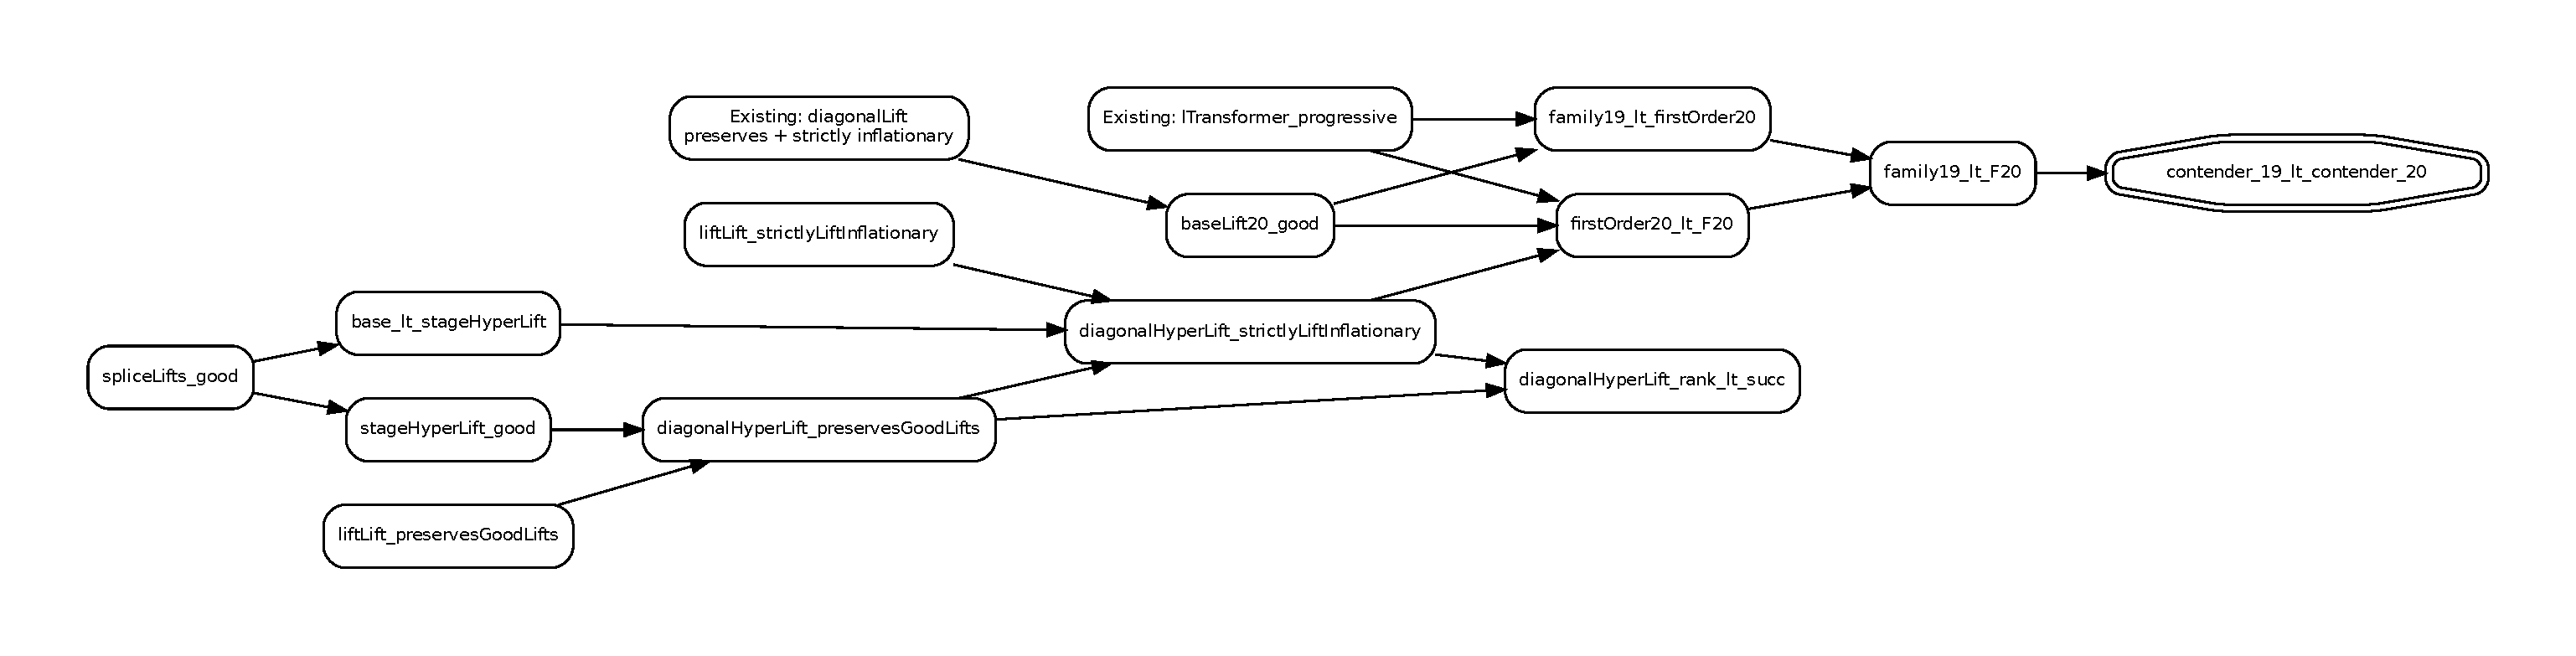
\includegraphics[width=\textwidth]{../figures/theorem_graph.pdf}
\caption{Dependency structure of the generic second-order facts and the final
Contender~20 comparison. Existing BusyLean theorems enter only through the two
leftmost nodes.}
\label{fig:theorem-graph}
\end{figure}

The graph highlights a useful separation of concerns.

\begin{itemize}[leftmargin=*]
\item The generic second-order library knows nothing about large-Veblen terms,
  \lean{F19}, or the closed contender.
\item The contender module supplies only schedule, rank, base lift, and seed.
\item The comparison module connects the generic facts to the existing
  \lean{lTransformer_progressive} theorem.
\end{itemize}

This modularity is important for future reuse. Any progressive reflection
transformer can replace \lean{lTransformer}, and any good transformer lift can
replace \lean{baseLift20}.

%======================================================================
\section{Computability and foundational hygiene}

\subsection{Structural recursion}

Every new computational definition recurses on an inductive datum:

\begin{center}
\begin{tabular}{lll}
\toprule
Definition & Recursion argument & Reason for termination\\
\midrule
\lean{stageHyperLift} & \leancode{WTree Nat} & structural recursion on the tree\\
\lean{diagonalHyperLift} & \lean{Nat} & structural recursion on the rank\\
\lean{schedule20} & inherited constructors & composition of existing total functions\\
\lean{F20} & none & finite composition of total definitions\\
\bottomrule
\end{tabular}
\end{center}

Countable branching does not threaten computability. A W-tree node stores a
function producing a child when a coordinate is requested; an evaluation uses
only the finitely many coordinates demanded by its finite computation.

\subsection{Forbidden mechanisms}

The supplied source-hygiene audit strips comments and rejects executable
occurrences of

\begin{center}
\lean{sorry}, \lean{admit}, \lean{axiom}, \lean{noncomputable},
\lean{unsafe}, \lean{partial}, \lean{opaque}, \lean{extern},
\lean{implemented_by}, and \lean{Classical.choice}.
\end{center}

The recorded audit result is \texttt{PASS}. This is not a substitute for a
kernel build, but it documents the intended constructive discipline.

\subsection{No oracle monotonicity assumption}

A tempting but invalid proof strategy would be to claim that a larger oracle
family always produces a larger reflected value. Reflected programs can inspect
oracle answers and branch, so output need not be monotone. The proposal follows
the existing repository discipline instead:

\begin{enumerate}[leftmargin=*]
\item progressivity exposes a concrete seed value inside each transformed
  family;
\item splicing exposes a concrete selected child;
\item strictness follows a fixed child-zero path;
\item all final comparisons compose these explicit occurrences.
\end{enumerate}

This is why the proofs remain valid for arbitrary progressive transformers,
not only for a specially monotone object language.

%======================================================================
\section{How large is the increase?}

\subsection{What is formally established}

The kernel-level claim is exact and modestly stated:
\[
  \operatorname{contender}_{19}<\operatorname{contender}_{20}.
\]
More structurally, the formal proof establishes the pointwise sandwich
\[
  \operatorname{family}_{19}(n)
  < \operatorname{firstOrder}_{20}(n)
  < F_{20}(n),
\]
where the middle term is a complete first-order diagonal hierarchy with
predecessor-sized rank and a schedule syntactically generated from the
predecessor schedule by a predecessor-sized hyper-closure.

\subsection{Why this is more than another natural rank}

Suppose, schematically, that a transformer lift $L$ is an amplification rule on
transformers. Contender~19 constructs many such $L$'s and diagonalizes among
them, but the rank remains a natural-number recursion \emph{inside the type}
$\Tr\to\Tr$.

Contender~20 forms operators
\[
  H:(\Tr\to\Tr)\to(\Tr\to\Tr)
\]
and diagonalizes among those. The outer recurrence can use an entire lower
lift hierarchy as both its local operator and its seed. In analogy with
classical fast-growth constructions, this resembles moving from iterating a
fixed normal function to iterating a closure operator that itself manufactures
whole function hierarchies. The analogy is heuristic; the Lean theorem does not
assign a canonical ordinal index to these operators.

\subsection{Why no exact ordinal calibration is claimed}

The BusyLean construction combines several ingredients whose interaction is
not captured by a standard published hierarchy:

\begin{itemize}[leftmargin=*]
\item a strongly normalizing large-Veblen universe ladder;
\item dynamic oracle families;
\item W-tree schedules generated from language-defined trees;
\item transformer-level autonomous closure;
\item first- and second-order diagonal reuse;
\item ranks and schedules numerically controlled by the predecessor family.
\end{itemize}

Assigning a proof-theoretic ordinal would require a lower-bound interpretation
and a matching upper-bound analysis for this precise higher-order reflection
algebra. Any simple expression such as ``$f_\alpha$ for this named $\alpha$''
would currently be conjectural. The article therefore makes only the robust
structural comparison supported by the source.

\subsection{A useful lower-bound reading}

Even without an ordinal label, the formal intermediate witness yields a clear
lower-bound narrative. At input $n$, $F_{20}(n)$ exceeds:

\begin{enumerate}[leftmargin=*]
\item the complete predecessor family value \leancode{family19 n};
\item one application of a predecessor-sized \lean{diagonalLift} hierarchy to
  the large-Veblen reflection transformer;
\item that whole first-order layer after it has been installed as the base of a
  predecessor-sized second-order diagonal hierarchy.
\end{enumerate}

Thus the margin is internal and compositional, not merely a consequence of the
outer definition \leancode{F20 (F20 42)}.

%======================================================================
\section{Lean engineering considerations}

\subsection{Avoiding enormous reduction}

The main practical danger in BusyLean proofs is asking the elaborator or
simplifier to compare terms by normalizing a contender-sized expression. The
new modules avoid that pattern.

\begin{itemize}[leftmargin=*]
\item No proof uses \leancode{simp [F20]}, \lean{decide}, or arithmetic evaluation
  on \lean{family19}.
\item The final theorem uses only previously proved strict inequalities and
  \lean{Nat.lt_trans}.
\item Definitions are unfolded only at small algebraic interfaces such as
  \lean{spliceLifts} and one W-tree constructor equation.
\item The smoke test contains \texttt{\#check} and \texttt{\#print axioms}, never
  \texttt{\#eval} or \texttt{\#reduce}.
\end{itemize}

\subsection{Expected compilation profile}

The new code is about four hundred lines including documentation and smoke
checks. Its proofs are generic and recurse only over theorem parameters, not
concrete gigantic ranks. The concrete numeral \leancode{rank20 n} is passed as an
opaque argument to already compiled recursive definitions. Accordingly, the
expected elaboration cost is governed by the size of the proof terms, not by
the value of the contender.

This expectation must still be tested on Lean~4.34.0. The repository's timing
rules make build performance part of acceptance.

\subsection{Potential elaboration sensitivities}

Three local points deserve attention during the first build.

\begin{enumerate}[leftmargin=*]
\item Lean must accept the structurally recursive theorem equations for
  \lean{stageHyperLift_good} and \lean{base_lt_stageHyperLift}. They mirror
  accepted equations in \lean{HyperReflectionFacts}.
\item One \lean{change} statement relies on definitional reduction of
  \lean{spliceLifts}, \lean{spliceTransformers}, and the node equation of
  \lean{stageHyperLift}. If reducibility settings interfere, replace it with
  explicit local \lean{rfl} equalities.
\item Implicit inference must resolve the nested property predicates. All
  applications are fully staged enough that any repair should be a local type
  annotation, not a mathematical change.
\end{enumerate}

%======================================================================
\section{Integration and validation}

\subsection{Files to add}

\begin{longtable}{p{0.46\linewidth}p{0.46\linewidth}}
\toprule
Path & Purpose\\
\midrule
\endhead
\lean{BusyLean/SecondOrderReflection.lean} & second-order definitions\\
\lean{BusyLean/SecondOrderReflectionFacts.lean} & generic goodness and strictness proofs\\
\lean{BusyLean/Contender20.lean} & schedule, ranks, $F_{20}$, and closed contender\\
\lean{BusyLean/Comparison20.lean} & pointwise and closed comparison theorems\\
\lean{test/SecondOrderReflectionSmoke.lean} & API and axiom smoke checks\\
\bottomrule
\end{longtable}

Add the four library imports to \lean{BusyLean.lean}. A ready-to-apply patch is
included as \lean{busylean_contender20.patch}.

\subsection{Required build commands}

\begin{lstlisting}[language={}]
lake build BusyLean.Comparison20
lake env lean test/SecondOrderReflectionSmoke.lean
lake build
lake env lean test/Audit.lean
\end{lstlisting}

The first command gives the focused kernel check. The full build catches import
cycles, naming collisions, and project-wide timing regressions. The existing
audit should be extended if it enumerates accepted contender names explicitly.

\subsection{Validation actually completed}

The package-generation environment completed the following work:

\begin{enumerate}[leftmargin=*]
\item audited the incumbent source interfaces and current tree identifier;
\item generated the Lean overlay and patch;
\item ran the static forbidden-marker and declaration audit;
\item compiled this article to PDF;
\item rendered the PDF to images and inspected the pages;
\item generated package checksums.
\end{enumerate}

A Lean executable was not installed, and network installation of the pinned
4.34.0 binary was unavailable. Therefore no statement in this article should be
read as claiming that the supplied overlay has already passed a kernel build.
The mathematics is reduced to local generic lemmas, but the build commands above
remain mandatory.

%======================================================================
\section{Further research}

\subsection{Third and higher operator levels}

The next literal step is to define
\[
  \mathsf{UltraLift}=\HL\to\HL
\]
and repeat the same construction. Hand-writing every finite level is possible
but conceptually unsatisfactory. A more valuable project is a dependent family
of carriers
\[
  A_0=\Tr,\qquad A_{k+1}=A_k\to A_k,
\]
together with recursively defined goodness, splicing, tree stages, and strict
inflationarity. The challenge is to package the varying types so that a
runtime-selected finite level can still be collapsed to a natural number.

\subsection{Transfinite hyper-ranks}

Current ranks are natural numbers, although each rank can contain enormous
tree schedules. One could index hyper-ranks by the already formalized
large-Veblen order. A successful design would require a well-founded recursion
whose successor/limit behavior preserves the explicit-witness strictness
proofs. This may be a cleaner route to transfinite operator order than extending
the object-language atom ladder again.

\subsection{Combining operator order with stronger ordinal atoms}

Second-order hyperreflection is orthogonal to the choice of
\lean{lTransformer}. If BusyLean later formalizes a Bachmann--Howard,
Takeuti--Feferman, or stronger well-founded atom order, the new reflection
transformer can be substituted beneath \lean{baseLift20}. The second-order
library should require no change.

\subsection{Ordinal calibration}

A serious calibration program should separate four questions.

\begin{enumerate}[leftmargin=*]
\item What standard hierarchy embeds into one progressive reflection
  transformer over the large-Veblen ladder?
\item What closure corresponds to \lean{liftTransformer} and
  \lean{diagonalLift}?
\item What new closure is introduced by \lean{liftLift} and
  \lean{diagonalHyperLift}?
\item Can matching upper bounds be proved by assigning ordinal diagrams to
  transformer and hyperlift terms?
\end{enumerate}

Without both lower and upper bounds, named-ordinal estimates should remain
explicitly heuristic.

\subsection{A certified Lean-kernel reflection contender}

Longer term, BusyLean could internalize a finite fragment of Lean's kernel or a
small dependent type theory strong enough to verify the existing contender
modules. A bounded maximum over certified closed programs would subsume many
hand-designed object languages. The key research problem is preserving
constructive executability while avoiding circular soundness claims.

\subsection{Performance instrumentation}

The repository would benefit from a standard benchmark script recording:

\begin{itemize}[leftmargin=*]
\item clean focused build time for each comparison module;
\item maximum resident memory;
\item axiom reports for contender and comparison theorem;
\item source scan for forbidden constructs;
\item proof-term size and imported declaration count.
\end{itemize}

Such data would make future proposals easier to compare on engineering quality,
not only on mathematical ambition.

%======================================================================
\section{Conclusion}

Contender~20 advances BusyLean along the most direct structural axis left open
by Contender~19. The incumbent already has a powerful object language and a
first-order diagonal hierarchy of transformer lifts. The proposal does not
merely lengthen that natural rank. It promotes whole lift hierarchies to the
objects manipulated by a new hyperlift level, proves that the corresponding
second-order diagonal ranks preserve the exact strict-growth invariant needed
by the contest, and embeds a complete predecessor-sized first-order layer as an
explicit lower witness.

The resulting formal chain is simple to state:
\[
  \operatorname{family}_{19}(n)
  < \operatorname{firstOrder}_{20}(n)
  < F_{20}(n),
\]
and it yields
\[
  \operatorname{contender}_{19}<\operatorname{contender}_{20}.
\]
All definitions are structural and intended to remain within BusyLean's
constructive rules. The remaining task before acceptance is concrete rather
than conceptual: build the overlay with Lean~4.34.0, inspect its axiom report,
and verify that focused and full builds remain inside the repository's timing
budget.

%======================================================================
\appendix

\section{Public API summary}

\begin{longtable}{p{0.44\linewidth}p{0.48\linewidth}}
\toprule
Declaration & Role\\
\midrule
\endhead
\lean{HyperLift} & endomorphism of transformer lifts\\
\lean{spliceLifts} & countable coordinate-selectable splice of lifts\\
\lean{stageHyperLift} & W-tree traversal with a local hyperlift\\
\lean{liftLift} & autonomous rank-zero second-order lift\\
\lean{diagonalHyperLift} & natural-rank second-order diagonal hierarchy\\
\lean{GoodLift} & preservation plus strict inflationarity\\
\lean{PreservesGoodLifts} & hyperlift closure invariant\\
\lean{StrictlyLiftInflationary} & strict comparison at lift level\\
\lean{diagonalHyperLift_preservesGoodLifts} & goodness of every rank\\
\lean{diagonalHyperLift_strictlyLiftInflationary} & strictness of every rank\\
\lean{diagonalHyperLift_rank_lt_succ} & adjacent-rank strictness\\
\lean{family19} & pointwise predecessor family\\
\lean{schedule20} & predecessor-sized autonomous schedule\\
\lean{rank20} & predecessor-sized natural rank\\
\lean{baseLift20} & embedded first-order diagonal lift\\
\lean{firstOrder20} & numerical value of the embedded first-order layer\\
\lean{F20} & second-order contender family\\
\lean{contender_20} & proposed closed BusyLean contender\\
\lean{family19_lt_firstOrder20} & first strict witness\\
\lean{firstOrder20_lt_F20} & second strict witness\\
\lean{contender_19_lt_contender_20} & required closed comparison\\
\bottomrule
\end{longtable}

\section{Static audit scope}

The included Python audit is intentionally small and reviewable. It performs
textual checks after stripping Lean comments, confirms expected declaration
markers, verifies critical import edges, and writes hashes and results to JSON.
It cannot establish parsing, elaboration, termination, or theorem correctness.
Only Lean's kernel can do that. Its purpose is to prevent accidental delivery
of unfinished or explicitly nonconstructive source and to make package contents
reproducible.

\section{Selected references}

\begin{thebibliography}{9}

\bibitem{BusyLean}
BusyLean contributors.
\newblock \emph{BusyLean: name the biggest number, in Lean}.
\newblock \url{https://github.com/VladimirReshetnikov/BusyLean}, 2026.

\bibitem{Roux}
Cody Roux.
\newblock \emph{name-the-biggest-number}.
\newblock \url{https://github.com/codyroux/name-the-biggest-number}.

\bibitem{Aaronson}
Scott Aaronson.
\newblock \emph{Who Can Name the Bigger Number?}
\newblock \url{https://www.scottaaronson.com/writings/bignumbers.html}.

\bibitem{Lean4}
Leonardo de Moura and Sebastian Ullrich.
\newblock The Lean 4 theorem prover and programming language.
\newblock In \emph{Automated Deduction -- CADE 28}, LNCS 12699,
  pages 625--635. Springer, 2021.

\bibitem{Schuette}
Kurt Sch\"utte.
\newblock \emph{Proof Theory}.
\newblock Springer, 1977.

\bibitem{Pohlers}
Wolfram Pohlers.
\newblock \emph{Proof Theory: The First Step into Impredicativity}.
\newblock Springer, 2009.

\end{thebibliography}

\end{document}
